Throughout the history, mankind has always been fascinated with the physics laws governing the universe. The theory known as atomism was one of the first attempts to understand the nature of matter. The concept of atoms formulated by Leucippus of Abdera (5th century before the common era) and further pursued by Democritus initiated the search for the building blocks of nature~\cite{sep-atomism-ancient}. According to this theory, everything consists of "atoms" (in ancient Greek \foreignlanguage{greek}{ἄτομος} which means uncuttable) that are physically indivisible, and the rest of space is just void. 

It's astounding to consider that at the turn of the twentieth century (roughly, 2500 years after atomism was formulated), the structure of the atom remained unknown. The electron had just been discovered, and its behavior and characteristics were still poorly understood. Knowledge about particle physics was scarce. Particles like nuclei, protons, and neutrons were poorly understood~\cite{intro_particle_physics}. 
Further discoveries of radioactivity (in the year 1896) and radioactive elements (in the year 1898) by H. Becquerel and M. Skłodowska-Curie marked the gateway to the 20th-century physics. 

High energy physics aims to explore the smallest and largest scales of the universe, seeking out new discoveries from the tiniest particles to the largest objects in space.
The number of important discoveries that have been made in the twentieth century is truly remarkable. Eventually, in 1970 these findings led to the formulation of a mathematical model called the Standard Model~\cite{intro_particle_physics}.  It describes the strong, weak, and electromagnetic fundamental interactions\footnote{The interactions that are considered not to be reducible to more basic ones} between the particles. 
 
 
 This work aims to take the reader on a journey from the theoretical objectives of physics, to the often complex process of development and construction of a particles detector for a high-energy physics experiment.
 %Modern ways of conducting experiments often involve use of advanced engineering and software engineering.
 
\section{Standard Model and the strong interaction}

The standard model is one of the most successful physics theories to date. It has explained numerous results from experiments worldwide. The most notable predictions of the Standard Model are the Higgs boson, W and Z bosons, the gluon, and the top and charm quark.

The standard model contains 17 particles (summarized in Figure~\ref{fig_standard})  that are the smallest building blocks and are categorized into two groups: bosons and fermions. These groups are distinguished by their spin properties: fermions (characterized by half-integer spin) obey Fermi–Dirac statistics and bosons (integer spin) obey Bose–Einstein statistics. 

Fermions are divided into two classes: quarks, which interact with the strong nuclear force, and leptons, which do not interact with it. Up and down quarks are located at the heart of atoms, inside the protons and neutrons. The other four quarks are only observed in particle accelerator collisions.

The electron is the most recognized of the leptons. Other charged leptons, known as muons and taus, are only discovered in particle accelerators and cosmic rays from space. Furthermore, each of the mentioned leptons has its corresponding neutrino, which has no electrical charge and a very small mass.

In addition to the particles, the Standard Model includes three forces that govern the behavior of matter. These forces are electromagnetism, strong and weak nuclear forces. The force-transmitting particles are the photon (electromagnetism), the gluon (strong nuclear force), the W \& Z bosons (the weak force), and the Higgs boson.

\begin{figure}[!h]
\centering
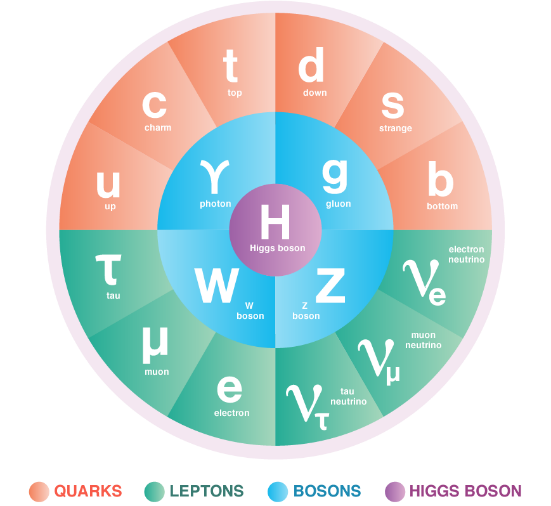
\includegraphics[width=0.7\columnwidth]{Chapter1/images/particles.png}
\caption{Fermions and bosons of the Standard Model~\cite{standard_model}.}
\label{fig_standard}
\end{figure}

\newpage

The Strong Force's theoretical foundation, Quantum Chromodynamics (QCD), is well established, with quarks and gluons describing the interaction between quarks mediated by gluons.

Yet, key phenomena in strong interactions, like the confinement of quarks and gluons into hadrons\footnote{Hadrons are composed of quarks, and therefore they experience the strong nuclear force} and the creation of mass, have remained unclear.

In extreme environments such as high-temperature T, or the high baryon density $\rho$, the confined baryonic matter may form a new state of matter called the quark-gluon plasma (\gls{QGP})~\cite{phase_diagram}. Hot deconfined matter dominated the early cosmos just a few microseconds after the Big Bang, but compact stars may also contain cold and baryon\footnote{Baryons are composed of three quarks, and they make up most of the visible matter in the universe.}-rich quark matter in their interiors.

A well-established non-perturbative approach to solving the quantum chromodynamics theory of quarks and gluons is known as the Lattice \gls{QCD}. LQCD can also be used to address issues like the confinement mechanism and chiral symmetry breaking, the role of topology, and the equilibrium properties of \gls{QCD} at finite temperature~\cite{lattice_qcd}. 

\section{Studies of nuclear matter and its forms}
 The phase diagram for nuclear matter is a representation of various phases, such as liquid, gas, or plasma. It also describes the borders between these states and types of transitions (see Figure~\ref{fig_phase}). The diagram illustrates the experimental results and theoretical predictions for the properties of nuclear matter.

The experimental search for \gls{QGP} in heavy ion
collisions was shaped by several model predictions of possible \gls{QGP} signals: suppressed production of charmonium states (bound states of a charmed quark and a charmed antiquark), in particular, $\mathrm{J/\psi}$ mesons, enhanced production of strange and multi-strange hadrons from the \gls{QGP}, characteristic radiation of photons and dilepton pairs from the \gls{QGP}. The results of the QGP search program at the \gls{CERN} The Super Proton Synchrotron \gls{SPS} on central collisions of medium and heavy nuclei were found to be adequate with the QGP predictions.

The crossover transition region was experimentally investigated at the Large Hadron Collider (\gls{LHC}) and Relativistic Heavy Ioc Colllider (\gls{RHIC}). This region is characterized by a low baryon chemical potential and high temperatures (around 150\,MeV), at which the ratio of baryons to antibaryons is almost equal. Lattice \gls{QCD} calculations show that the transition at $\mu_{B} = 0$ is a crossover transition~\cite{Aoki_2006}. Because there is no real phase transition, the crossover temperature is unclear, as alternative definitions might result in different results. The nuclear matter is expected to hadronize at the temperature of 155--160 MeV~\cite{Bazavov_2012, Stachel_2014}.



\begin{figure}[!h]
\centering
 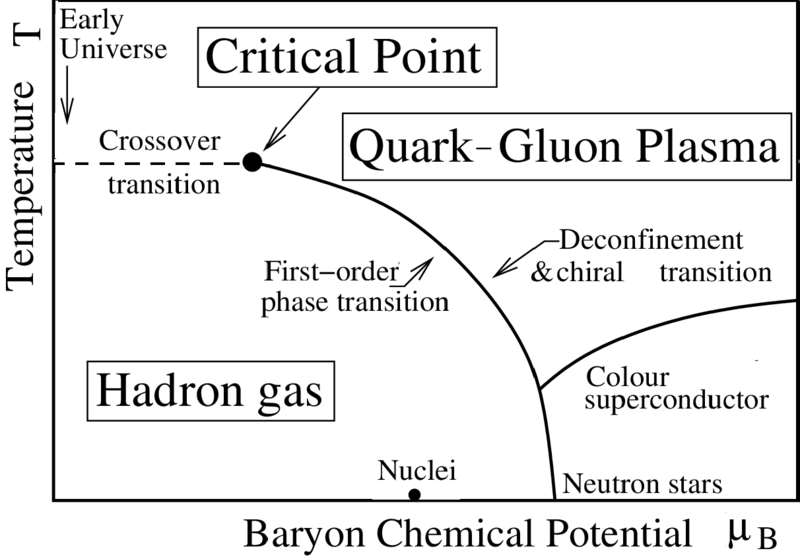
\includegraphics[width=0.65\columnwidth]{Chapter1/images/phase.png}
\caption{The phase diagram illustrating the regimes of confined and deconfined states of nuclear matter. The critical point separates the region of a cross-over (explored by \gls{RHIC} and \gls{LHC}) from that of a first-order phase transition to be studied by the CBM experiment~\cite{friese_diagram}.}
\label{fig_phase}
\end{figure}
\newpage
Figure \ref{fig_phase} also depicts structures at higher baryon-chemical potentials, such as a chiral and a deconfinement first-order phase transition merging at a critical point with a region of quarkyonic matter in between. To date, none of these structures or phases have been discovered. As previously stated, first-principles theories, such as perturbative QCD, continue to struggle to generate solid predictions for matter characteristics at higher baryon-chemical potentials~\cite{Sakai_2008, Fischer_01, Tawfik_01}. 


%\section{Physics goa}

\section{Probing dense nuclear matter with heavy ion collisions}

Heating or compressing nuclear matter leads to the deconfined state of matter when the temperature and density exceed a threshold point, as denoted in Figure~\ref{fig_phase}. Heavy ion collisions in the beam energies between \agev{2} and \agev{11} have an enormous potential to explore many aspects of the phase diagram. Figure \ref{fig:cbm_density} represents the time evolution of a Au+Au collision system at \agev{10} energy. Such conditions are expected to dominate during the supernovae core collapse and in the core of neutron stars. Furthermore, the calculations of different transport models and hydrodynamics show that the density of the fireball will reach more than $8\rho_{0}$ during the Au+Au collisions at \agev{10}~\cite{CBM_physics}.
\newpage
\begin{figure}[!h]
    \centering
    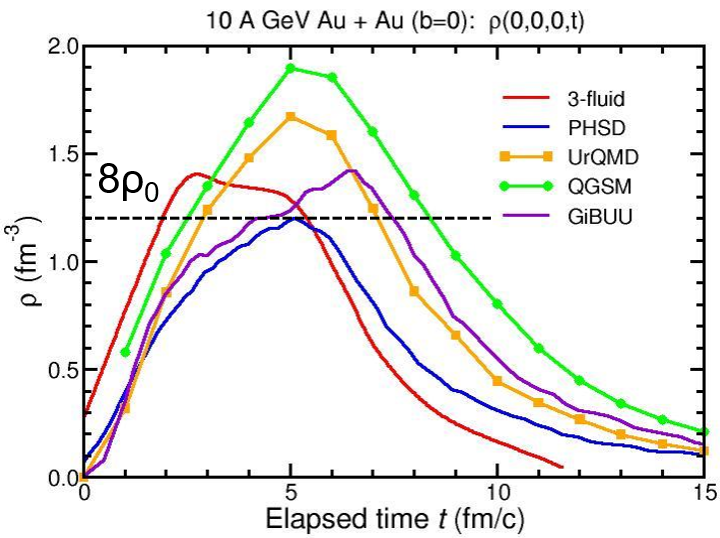
\includegraphics[width=0.65\columnwidth]{Chapter1/images/CBM_density.png}
    \caption{The time evolution of the central net baryon density $\rho(t)$ calculated using different transport models and 3-fluid hydrodynamics of a head-on Au+Au collision at \agev{10} energy (indicated in \agev{})~\cite{CBM_physics}.}
    \label{fig:cbm_density}
\end{figure}

Figure~\ref{fig_heavyion} depicts the presumed evolution of the heavy ion collision. As mentioned before, the creation of the \gls{QGP} depends mostly on the conditions (temperature and pressure) of the colliding particles. It illustrates the various forms of QCD matter intervening during the subsequent phases of the collision for hadronic collisions and heavy ion collisions.
\begin{figure}[!h]
\centering
 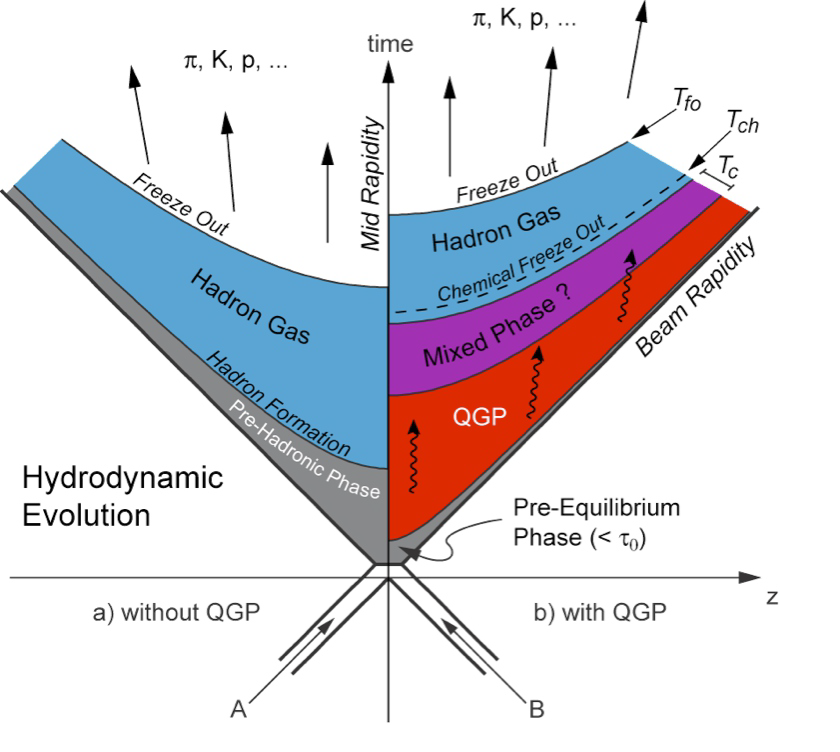
\includegraphics[width=0.6\columnwidth]{Chapter1/images/heavyion.png}
\caption{Schematic representation of the various stages of a HIC as a function of time t and the longitudinal coordinate z (the collision axis). The critical temperature is represented by $T_c$, whilst the freeze-out and chemical freeze-out temperatures are indicated by $T_{fo}$ and $T_{ch}$, respectively~\cite{Sahoo:2745520}.}
\label{fig_heavyion}
\end{figure}

 After the collision (right side of the graph in Figure~\ref{fig_heavyion}), the system enters a pre-equilibrium phase, followed by a deconfined QGP medium and a probable mixed phase (which should exhibit first-order phase transition signals).

Heavy ion experiments around the world have been exploring the facets of the phase diagram through systems characterized by a wide range of temperatures and densities. Figure~\ref{fig:cbm_rates} shows the interaction rates of existing and planned heavy-ion experiments. Groundbreaking heavy-ion experiments at AGS in Brookhaven and at low CERN-SPS beam energies have investigated the QCD phase diagram at large baryon chemical potentials. Because of the detector technologies available at the time, these observations were limited to abundantly generated hadrons and di-electrons with severely constrained statistics. The NA61/SHINE experiment at CERN-SPS has been searching for the first-order phase transition by investigating hadrons with light and heavy ion beams~\cite{CBM_physics, Turko:2301677}.

The studies conducted at the Solenoidal Tracker at \gls{RHIC} (\gls{STAR}) and A Large Ion Collider Experiment (\gls{ALICE}) at \gls{LHC} revealed that the partonic degrees of freedom prevail at the early phase of the fireball evolution~\cite{CBM_physics}.

The HADES detector at SIS18 detects hadrons and electron pairs in heavy-ion collision systems at reaction rates of up to \khz{20} and beam energy of 1-\agev{2}~\cite{Ablyazimov_2017}.


The STAR Collaboration at \gls{RHIC} has
performed a beam energy scan from top energies down
to $\sqrt{s_{NN}} =$~\gev{7.7}, where $\sqrt{s_{NN}}$ is the center of mass energy of two colliding nuclei N.  The Beam Energy Scan (\gls{BES}) phase I program findings indicate evidence of a first-order phase transition in the QCD phase diagram and the turn-off of the quark gluon plasma's distinctive fingerprints at low collision energy. BES phase II program (BES II) covers the $\sqrt{s_{NN}}$ from \agev{7.7} to \agev{19.6} in the collider mode and from \agev{3} to \agev{7.7} in the fixed-target mode~\cite{STAR2, STAR1}.

The Nuclotron at the Joint Institute for Nuclear Research (JINR) in Dubna is preparing the fixed-target experiment BM@N to explore heavy-ion collisions at gold beam energy up to roughly \agev{4}. Furthermore, the Nuclotron-based Ion Collider fAcility NICA with the Multi-Purpose Detector (MPD) is being built at JINR. The NICA collider is intended to operate at collision energies ranging from $\sqrt{s_{NN}} =$~\agev{8} to \agev{11}, with reaction rates up to \khz{6} for minimal bias Au+Au collisions~\cite{Ablyazimov_2017}.

\begin{figure}[!h]
    \centering
    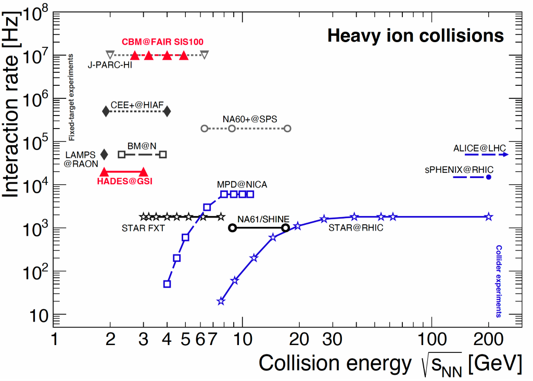
\includegraphics[width=0.7\columnwidth]{Chapter1/images/interaction_rates.png}
    \caption{Interaction rates achieved by existing and planned heavy-ion experiments as a function of the center-of-mass energy. “STAR FXT” denotes the fixed-target operation of STAR.  Blue symbols show collider experiments, black and gray symbols show fixed-target experiments~\cite{Ablyazimov_2017}.}
    \label{fig:cbm_rates}
\end{figure}




\gls{CBM} is a fixed target experiment that aims to measure rare particles as probes of dense matter with very good precision at beam energies up to \agev{11} or $\sqrt{s_{NN}}$ = \gev{4.9} (up to \agev{14} for light nuclei and \agev{29} for protons) and interaction intensities up to 10~MHz.
\newpage
It is well positioned to explore many facets of \gls{QCD} matter and to discover new exotic states. In addition, it will be able to explore the equation of state at densities (2–6 times saturation density) and temperatures close to those probed by cores of massive neutron stars, supernovas and in neutron star mergers~\cite{Senger_2020}. The majority of the experimental observables which are sensitive to the properties of dense nuclear matter, like the flow of (anti-) particles, higher moments of event-by-event multiplicity distributions of conserved quantities, multi-strange (anti-) hyperons, di-leptons, and particles containing charm quarks are prone to the statistics. Therefore, the key feature of successful experiments is high rate capability, that ensures high precision~\cite{Ablyazimov_2017}. 

The \gls{CBM} aims to investigate:
\begin{enumerate}
    \item the equation of state of baryonic matter at neutron star densities,
    \begin{itemize}
        \item collective behavior and flow anisotropies - the collective hadrons motion provides the information on the dense stage of the heavy ion collision. It's driven by the pressure gradient created at the beginning of the fireball evolution~\cite{Reisdorf_2007},
        \item hyperons and their interactions - are preferentially produced in the dense phase of the fireball via sequential collisions.
    \end{itemize}
    \item modifications of hadron properties in the dense baryonic matter and the onset of chiral symmetry restoration. These phenomenons affect the invariant-mass spectra of di-leptons, which will be measured both in the electron and the muon channel,
    \item phase transitions from hadronic matter to quarkonic or partonic matter:
    \begin{itemize}
        \item the excitation function of multi-strange hyperons, which are driven into equilibrium at the phase boundary,
        \item the excitation function of the invariant mass spectra of lepton pairs which reflect the fireball temperature, and, hence, may reveal a caloric curve and a first-order phase transition,
        \item the excitation function of higher-order event-by-event fluctuations of conserved quantities such as strangeness, charge, and baryon number are expected to occur in the vicinity of the critical point.
    \end{itemize}

     
     
    \item hypernuclei (double $\Lambda$, strange di-baryons etc.) and the measurement of their lifetime will provide information on the hyperon-nucleon and hyperon-hyperon interaction,
    \item charm production mechanisms.
\end{enumerate}
A detailed description and explanation of the \gls{CBM} physics program can be found in the \gls{CBM} Physics Book~\cite{CBM_physics} and in~\cite{Ablyazimov_2017}.



